\chapter{Anhang}
\section{Bilder}
% TODO: Bilder insertFirst Good (4)
% TODO: Bilder insertFirst Bad (4)
% TODO: Bilder insertFurthest Good (5)
% TODO: Bilder insertFurthest Bad (5?)
% TODO: Merge Algorithmus in Anhang


% \section{Subtestanhang}

% \chapter{Noch ein Testanhang}

% -------------------------------------------------------------- 
% INSERT CLOSEST BAD COMPLETE
\begin{figure}[h]
    \begin{center}
        \subfloat[$m = 2$\label{app:subfig:insert-closest-BAD-m1}]{%
        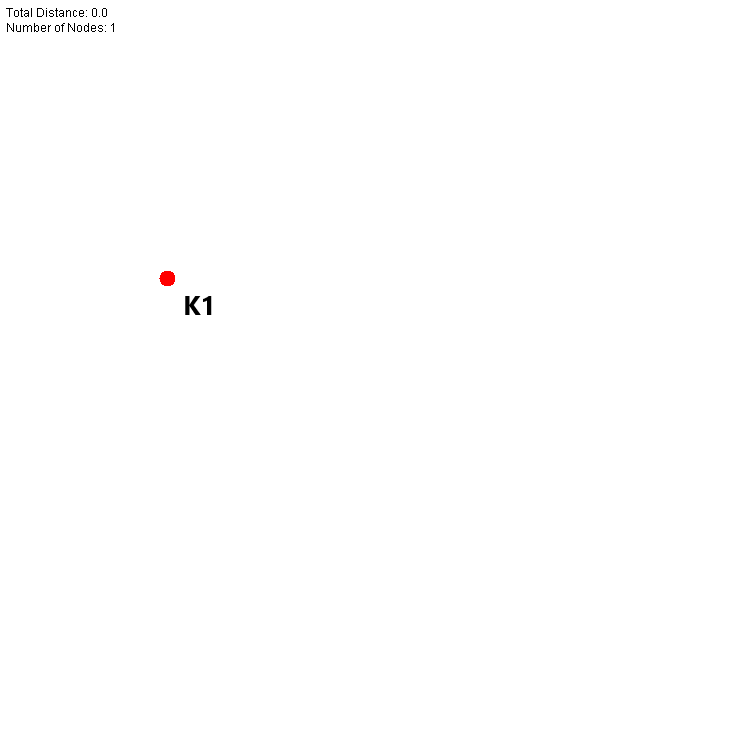
\includegraphics[width=0.6\textwidth]{./Bilder/insertClosest/insert_closest_ex_BAD_1.PNG}
        }
    \end{center}
\end{figure}
\begin{figure}\ContinuedFloat
    \begin{center}
        \subfloat[$m = 3$\label{app:subfig:insert-closest-BAD-m2}]{%
        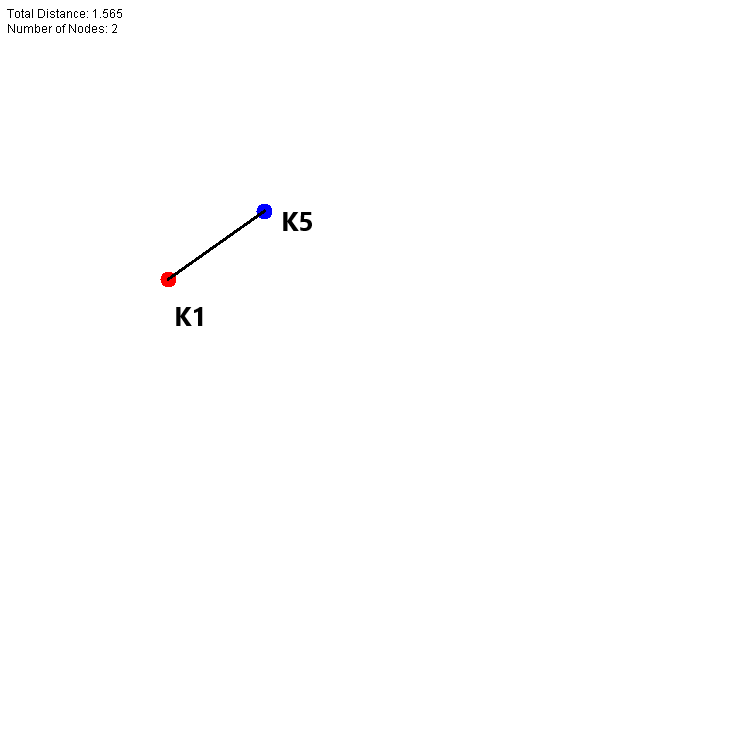
\includegraphics[width=0.6\textwidth]{./Bilder/insertClosest/insert_closest_ex_BAD_2.PNG}
        }
    \end{center}
\end{figure}
\begin{figure}\ContinuedFloat
    \begin{center}
        \subfloat[$m = 4$\label{app:subfig:insert-closest-BAD-m3}]{%
        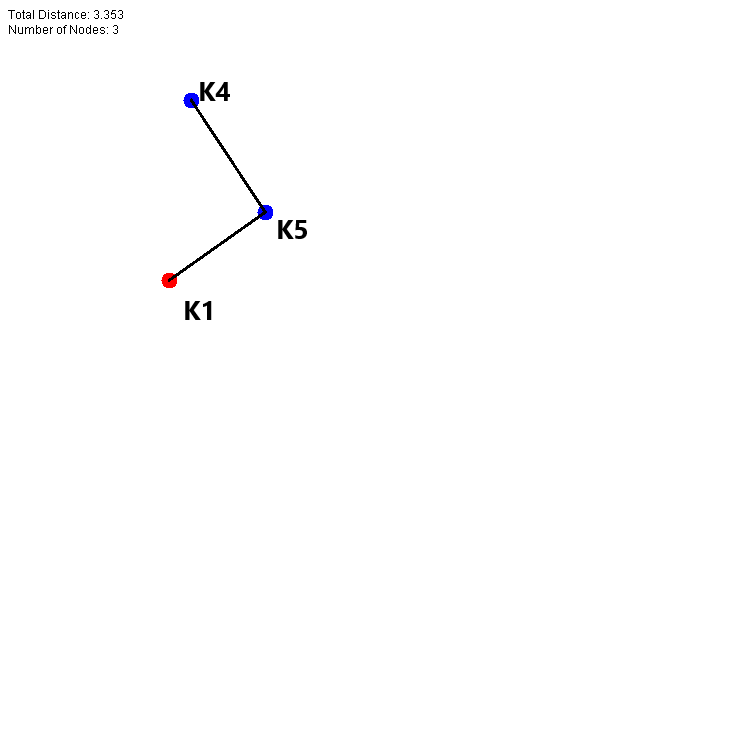
\includegraphics[width=0.6\textwidth]{./Bilder/insertClosest/insert_closest_ex_BAD_3.PNG}
        }
    \end{center}
\end{figure}
\begin{figure}\ContinuedFloat
    \begin{center}
        \subfloat[$m = 5$\label{app:subfig:insert-closest-BAD-m4}]{%
        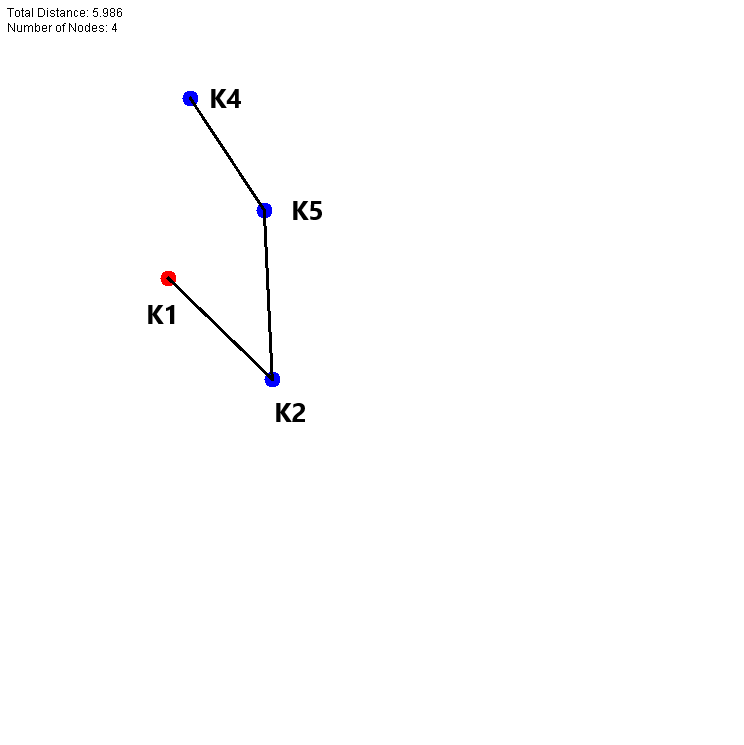
\includegraphics[width=0.55\textwidth]{./Bilder/insertClosest/insert_closest_ex_BAD_4.PNG}
        }
    \end{center}
\end{figure}
\begin{figure}\ContinuedFloat
    \begin{center}
        \subfloat[$m = 5$\label{app:subfig:insert-closest-BAD-m5}]{%
        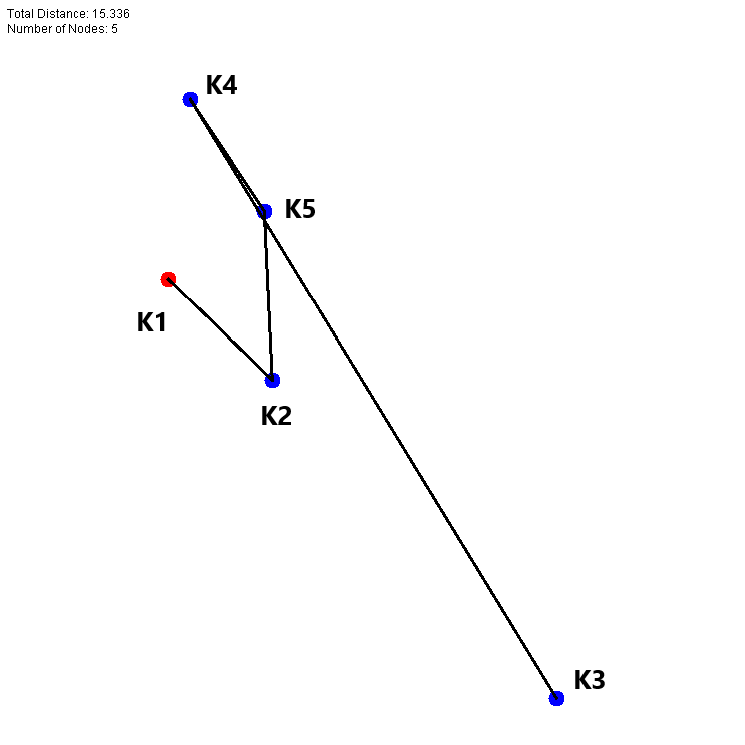
\includegraphics[width=0.55\textwidth]{./Bilder/insertClosest/insert_closest_ex_BAD_5.PNG}
        }
        \caption{Viele Bilder}
    \end{center}
\end{figure}
\label{app:fig:insert-closest-BAD-complete}

% -------------------------------------------------------------- 
% Crossover Example 40 Nodes
\begin{figure}[h]
    \begin{center}
        \subfloat[Pfad mit einem Crossover\label{app:subfig:40-nodes-with-crossover}]{%
        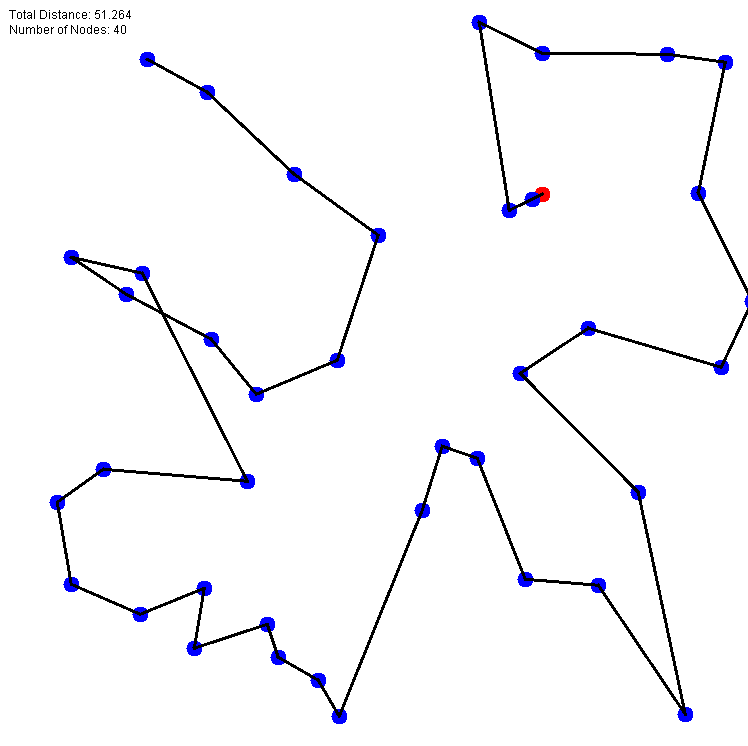
\includegraphics[width=0.55\textwidth]{./Bilder/crossover/40_nodes_with_crossover}
        }
    \end{center}
\end{figure}
\begin{figure}\ContinuedFloat
    \begin{center}
        \subfloat[Pfad mit aufgelöstem Crossover\label{app:subfig:40-nodes-without-crossover}]{%
        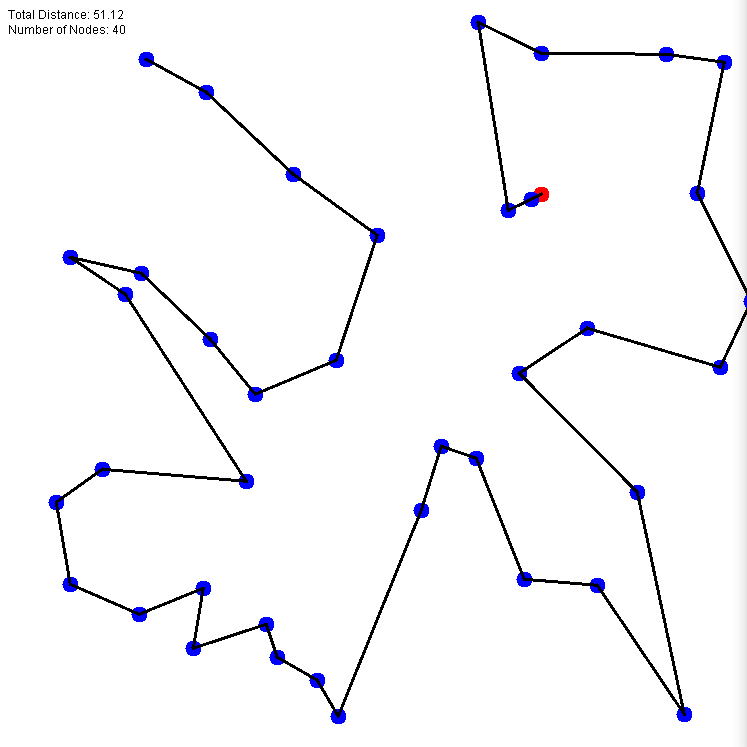
\includegraphics[width=0.55\textwidth]{./Bilder/crossover/40_nodes_without_crossover.PNG}
        }
        \caption{Pfad aus 40 Knoten mit und ohne Crossover}
    \end{center}
\end{figure}\label{app:fig:40-nodes-crossover-example}

\section{Algorithmen}
\begin{algorithm}[h]
    \caption{Einfügen eines Knoten in einen Pfad}
    \label{alg:merge-node-into-path}
    \begin{algorithmic}[1]
        \Require Pfad $P = K_1,\ldots,K_n$
        \Require Knoten $K^*$, Index $i$, $i \leq n$
        \For{$a \gets n$, $a \geq i$, $a \gets a+1$}
            \State $P_{a+1} \gets P_a$
        \EndFor
        \State $P_i \gets K^*$ \\
        \Return $P$
    \end{algorithmic}
\end{algorithm}

